\documentclass{article}
\usepackage{geometry}
 \geometry{
 a4paper,
 total={170mm,257mm},
 left=20mm,
 right=20mm,
 top=15mm,
 }
\usepackage{times}
\usepackage{graphicx}
\usepackage{url}

\graphicspath{{figures/}}

\begin{document}

\title{Evaluation of Video Quality Assessment Algorithms}
\author{Sophie M Greene}

\maketitle

\begin{abstract}
Since human subjects are the end users of videos, they are considered the most reliable in evaluating video quality. Hence, the most accurate video quality assessment method is the subjective Mean Opinion Square MOS, which is acquired using human subjects in a controlled viewing environment, this process is time consuming and expensive, thus the need for computational models that can predict perceived video quality accurately and automatically. These computational models are commonly known as objective Video Quality Assessment VQA algorithms and they have many applications commercially and otherwise.
This report describes a set of experiments conducted to evaluate the different existing objective VQA algorithms using a subjective study of the same videos. The video sequences were acquired from LIVE Video Quality Database ~\cite{kalp2010a,kalp2010b}; which consist of 10 original videos as well as 15 distorted copy of each. The distortion methods vary from compression to simulated transmission over different communication channels. The Peak Signal to Noise Ration PSNR, Structural Similarity Index SSIM and the Visible Signal to Noise Ratio VSNR objective algorithms are applied to the videos and the outcome of each is plotted against the corresponding subjective scores. Finally, the Spearman Rank Order Correlation Coefficient SROCC and Pearson Linear Correlation coefficient LCC are computed to evaluate the relationship between the aforementioned objective algorithms and the subjective scores. The results of the evaluation are compared to study in ~\cite{kalp2010a,kalp2010b}.
\end{abstract}

\section{Introduction}
\label{sec:intro}
During acquisition, processing, compression, storage, transmission and reproduction, digital videos are subject to a wide variety of distortions which could cause a degradation of the videos' visual quality. In applications where human beings are the ultimate viewers of videos, subjective evaluation is the most reliable method for quantifying visual video quality. However, subjective evaluation is costly and time consuming thus the need for automated video quality assessment VQA algorithms to provide quantitative measures capable of predicting the perceived video quality. Objective VQA metrics can play a variety of roles in video processing applications; one of which is dynamically monitoring and adjusting video quality. For example, a TV channel broadcasting live over the Internet can examine the quality of video being transmitted and allocate streaming resources accordingly. VQA metrics can also be used to optimise algorithms and parameter settings of video processing applications.
Objective VQA metrics can be classified according to many criteria. In this context, the criterion we are interested in is the availability of an original, distortion-free video, with which the distorted video is compared. A VQA metric is referred to as full-reference FR whenever a complete reference video is available. Practically, the reference video is not always available, which inspires video quality assessment algorithms that try to quantify the quality of a video without a reference video being available, this approach is referred to as no-reference NR, VQA algorithm. Reduced Reference RF is the third class of VQA algorithms in which the reference video is only partially available in the form of a subset of features from the original video used to judge the quality of a distorted one. For more on VQA algorithms classification refer to~\cite{wang2006}.
For any objective VQA algorithm to be truly successful, it needs to be validated. Our experiments aim to validate and inspect the effectiveness of some of the most commonly used FR VQA such as PSNR, SSIM, MS-SSIM and VSNR.
Section ~\ref{subjective} describes the the videos used in the experiment  and the subjective video quality assessment measure, the Difference Mean Opinion Score DMOS and the procedure used to calculate this measure . Section ~\ref{objective} descibe the objective VQA algorithms being validated. in section ref 


\section{Subjective Video Quality Assessment}
\label{sec:subjective}
Since human beings are the ultimate receivers in most video processing applications, the most reliable way of assessing the quality of an image is by subjective evaluation. Indeed, the mean opinion score (MOS), a subjective quality measure requiring the services of a number of human observers, has been long regarded as the best method of image quality measurement.
\subsection{Reference Videos}
The reference videos are ten uncompressed videos available from~\cite{kalp2010a}in uncompressed planner YUV 4:2:0 format, the each of the videos has a 768x432 pexils resolution.
\begin{figure}[h]
    \centering
    \begin{tabular}[h]{cc}
        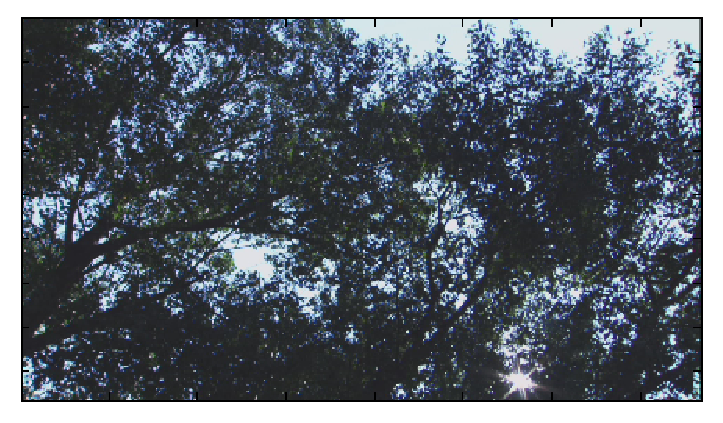
\includegraphics[scale=.55]{orig} &
        
\includegraphics[scale=.55]{wireless} \\
        (a)~Original frame&
        (b)~wireless loss simulated frame \\
       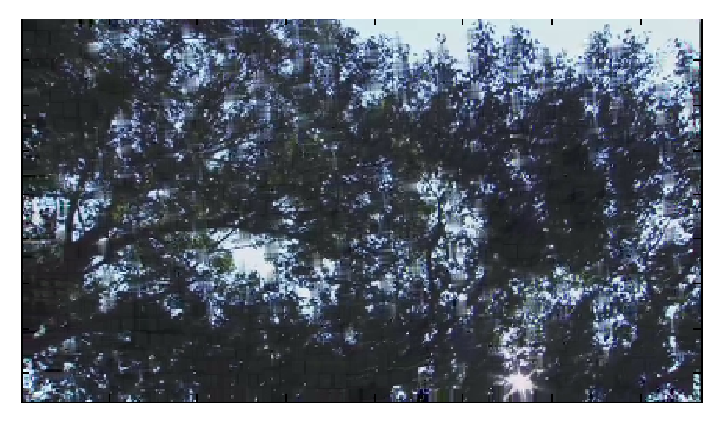
\includegraphics[scale=.55]{ip} &
       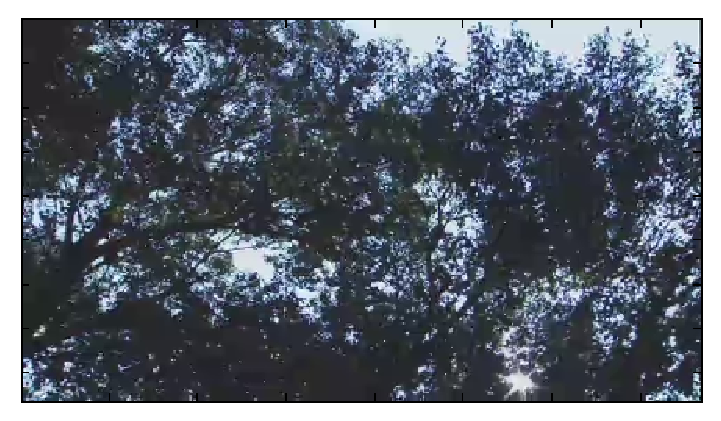
\includegraphics[scale=.55]{h264} \\
        (c)~IP loss simulated frame&
        (d)~H.264 compressed frame
    \end{tabular}
    \caption{Examples of distorted frames.}

    \label{fig:frames}
\end{figure}

\subsection{Distorted Videos}
We used 15 distorted videos for each reference video. the videos were created using four different distortion processes - MPEG-2 compression (4 test videos per reference), H.264 compression (4 test videos per reference), lossy transmission of H.264 compressed bitstreams through simulated IP networks (3 test videos per reference) and lossy transmission of H.264 compressed bitstreams through simulated wireless networks (4 test
videos per reference)~\cite{kalp2010a,kalp2010b}.Figure~\ref{fig:frames} illustrates sample frames from the reference and distorted videos.
\subsection{Difference Opinion Mean Square DMOS}
we used the DMOS scores provided by~\cite{kalp2010a} which were obtained by the following procedure
\begin{enumerate}
    \item in two half-hour sessions; show a playlist consisting of the test and reference videos to 38 participants, asking them to rate each video after it is displayed. The rating categories are ``Excellent'', ``Good'', ``Fair'', ``Poor'' and ``Bad''.
    \item Compute the difference score for each of the test videos by subtracting each score from each corresponding reference video.
    \item The difference scores were then normalised by subtracting  the mean of the scores assigned by the participant in the session from each difference score and dividing the result by the standard deviation of scores assigned by the participant in the corresponding session.
    \item The results were statistically manipulated to check for outliers and scores from 9 participants were rejected
    \item The remaining normalised scores were re-scaled in the range [1:100]
    \item The DMOS of each video was computed as the mean of the re-scaled normalised scores
\end{enumerate}


\section{Objective Video Quality Assessment}
\label{sec:objective}
The goal of objective image quality assessment research is to design computational models that can predict perceived image quality accurately and automatically. We use the term predict here, since the numerical measures of quality that an algorithm provides are useless unless they correlate well with human subjectivity. In other words, the algorithm should predict the quality of an image that an average human observer will report.
Objective VQA metrics can be classified according to many criteria. The criterion we are interested in, in this context, is the availability of an original, distortion-free video, with which the distorted video is compared. Reduced Reference RF is the third class of VQA algorithms in which the reference video is only partially available in the form of a subset of features from the original video used to judge the quality of a distorted one. A VQA metric is referred to as full-reference FR whenever a complete reference video is available. Practically, the reference video is not always available, which inspires video quality assessment algorithms that try to quantify the quality of a video without a reference video being available, this approach is referred to as no-reference NR, VQA algorithm. For more on VQA algorithms classification refer to~\cite{wang2006}.

\subsection{Peak Signal to Noise Ratio PSNR}

Equation~\ref{eqn:psnr} defines the peak signal to noise ratio.

\begin{equation}
\label{eqn:mse}
   MSE =
   \frac {1}{N}{
        \sum_{i=1}^{N} |x_i-y_i|^2
    }
\end{equation}
\begin{equation}
\label{eqn:psnr}
  PSNR = 10
    \log_{10}{\frac{L^2}{MSE}}
\end{equation}
\subsection{Structural Similarity Index SSIM}
Natural image signals are highly structured. Samples taken from image signals have strong dependencies amongst themselves, and these dependencies carry important information about the structures of the objects in the visual scene.The principal idea underlying the structural similarity approach is that the HVS is highly adapted to extract structural information from visual scenes, and therefore, a measurement of structural similarity (or distortion) should provide a good approximation to perceptual image quality.

\begin{figure}[h]
    \centering
    \begin{tabular}[h]{cc p{20em} p{20em}}
        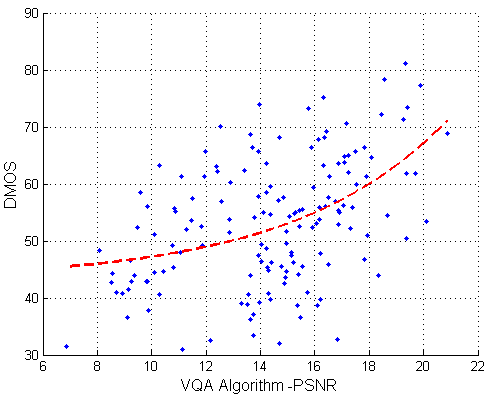
\includegraphics[scale=.45]{psnr} &
        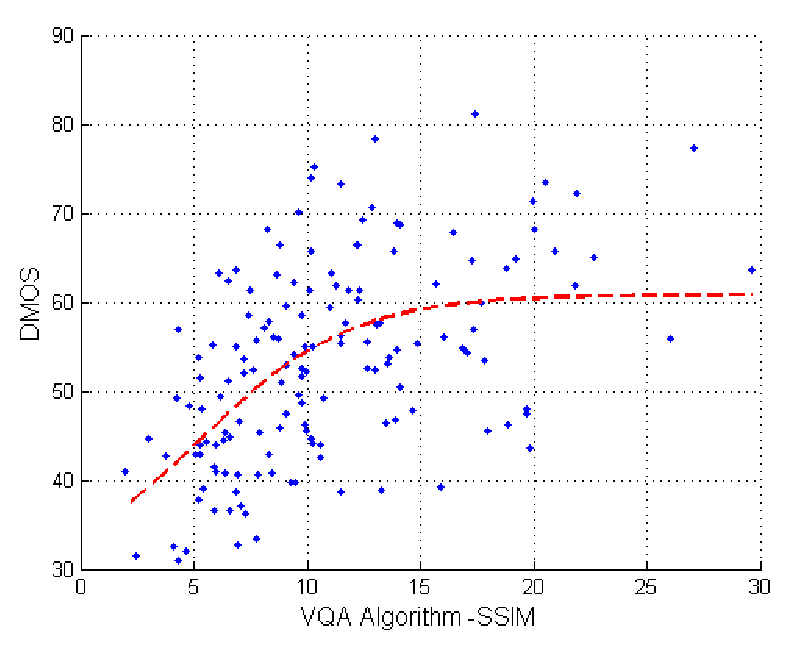
\includegraphics[scale=.45]{ssim} \\
        (a)~a PSNR vs DMOS &
        (b)~SSIM vs DMOS \\
       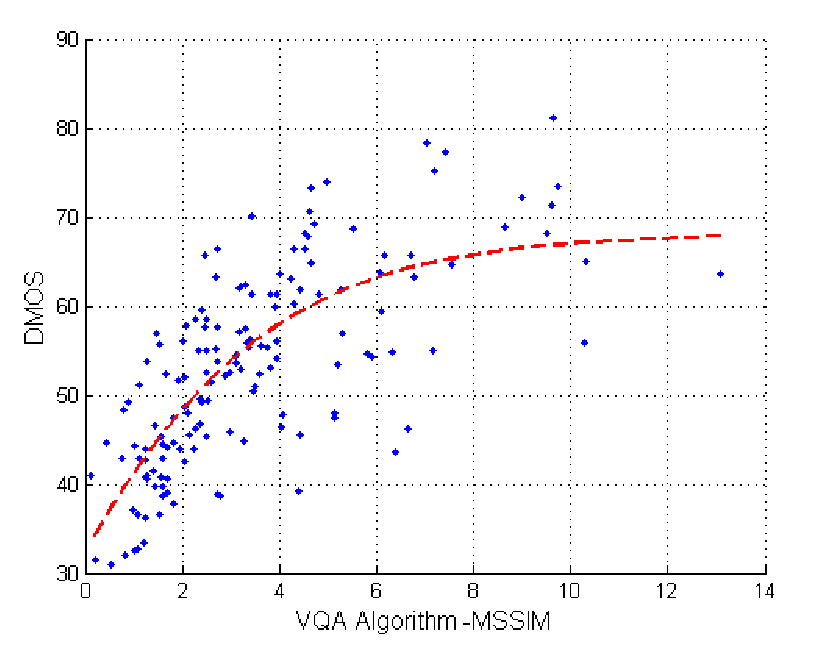
\includegraphics[scale=.45]{msssim} &
       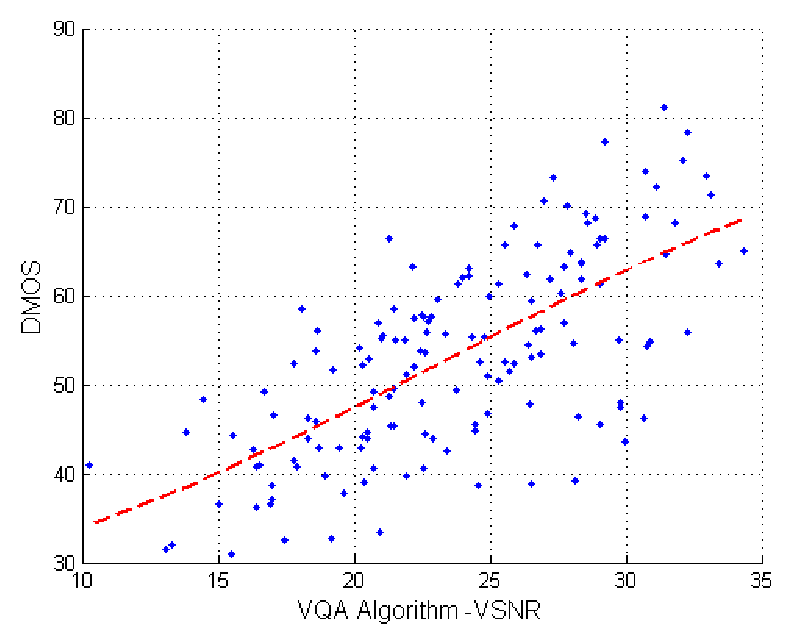
\includegraphics[scale=.45]{vsnr} \\
        (c)~MS-SSIM vs DMOS&
        (d)~VSNR vs DMOS
    \end{tabular}
    \caption{Evaluation of different objective VQA. a plot showing the relationship. small values of DMOS indicates a good quality of the video assessed while }
    \label{fig:vqa}
\end{figure}
\begin{table}
\centering
\begin{tabular}[h]{ p{10em}  p{5em}  p{5em}}
\hline\hline
			VQA & SROCC & LCC \\\hline
			PSNR & 0.4268 &0.4617 \\ 
			VSNR &0.6731   & 0.6889 \\ 
			SSIM &0.5209  &0.5384 \\ 
			MSSIM & 0.7349 & 0.6812 \\	\hline\hline
 \end{tabular}
    \caption{SROCC \& LCC}
  \end{table}
\bibliographystyle{plain}
\bibliography{local}
\end{document}
